\documentclass[compress,10pt,aspectratio=169]{beamer}
%\setbeamertemplate{background canvas}[bottom=white,top=structure.fg!25]
%\usetheme{Hannover}
%\setbeamertemplate{headline}{}
%\setbeamertemplate{footline}{}
\setbeamersize{text margin left=0.1cm}
\usepackage{appendixnumberbeamer}
\usepackage{hyperref,listings,picinpar,mathtools} % ,enumitem}
\usepackage{color}
\settowidth{\leftmargini}{\usebeamertemplate{itemize item}}
\addtolength{\leftmargini}{\labelsep}
\usepackage{fancyvrb}
%\usepackage{xcolor}
\beamertemplatenavigationsymbolsempty

\definecolor{grey}{rgb}{0.95,0.95,0.95}
\definecolor{red}{rgb}{1.0,0.0,0.0}
\definecolor{green}{rgb}{0.0,0.6,0.0}
\definecolor{blue}{rgb}{0.0,0.0,1.0}
\lstloadlanguages{bash,Java,C,C++,csh,make,sh}%%[Visual]Basic,xml}
\lstset{frame=none,basicstyle=\tiny,breaklines,tabsize=2,captionpos=b,prebreak={\hbox{$\rightarrow$}},postbreak={\hbox{$\hookrightarrow$}},showstringspaces=false,backgroundcolor=\color{grey}\bfseries,keywordstyle=\color{blue},commentstyle=\color{green}\textit,stringstyle=\color{red}\ttfamily,abovecaptionskip=2pt,aboveskip=0pt,belowskip=0pt,belowcaptionskip=0pt}
%\lstset{moredelim=[is][\color{red}]{_+_}{_+_}}

\beamertemplatefootpagenumber
% \setbeamertemplate{footline}[page number]{}
%\setbeamertemplate{page number in head/foot}{}

\setbeamertemplate{footline}[text line]{\hspace*{15.6cm}\insertpagenumber}
\setbeamertemplate{navigation symbols}{}

\usepackage{graphicx,verbatim,multicol,amsmath,bm}
\graphicspath{{./figures/}{../pictures/}}

\title{Synchronizing SDR and other clocks on white rabbit}
\author{\'Emilien Decoux, Jean-Michel Friedt\\ \ \\ 
FEMTO-ST Time \& Frequency department, Besan\c con, France \\ \ 
\\ \ \\ emilien.decoux@edu.univ-fcomte.fr, jmfriedt@femto-st.fr \ \\ \ \\
%project archive at \url{https://github.com/oscimp/wr_acorn}\\
%\vspace{-1.27cm}
\parbox{1.0\linewidth}{
\includegraphics[width=.3\linewidth]{logo_femtost.pdf}\hfill

\includegraphics[width=.27\linewidth]{WR_logo_on_white}}\vspace{-1cm}  
}

\begin{document}
\maketitle

\begin{frame}[fragile]\frametitle{Syntonising RF SOCs on White-Rabbit}

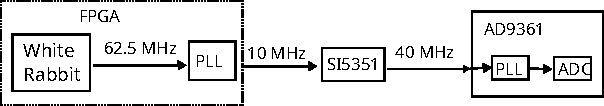
\includegraphics[width=\linewidth]{m2sdr_syntonized_fig.pdf}

\end{frame}

\begin{frame}[fragile]\frametitle{PLL Indeterminism}

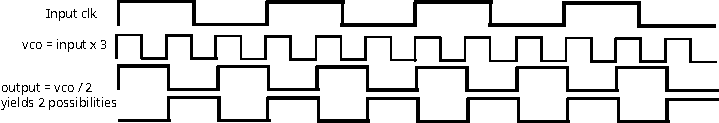
\includegraphics[width=\linewidth]{pll_indeterminism_fig.pdf}
PLL multiplying by 1.5, division by 2 yields 2 possible phase positions.


\end{frame}

\begin{frame}[fragile]\frametitle{Auxiliary Locksweep}

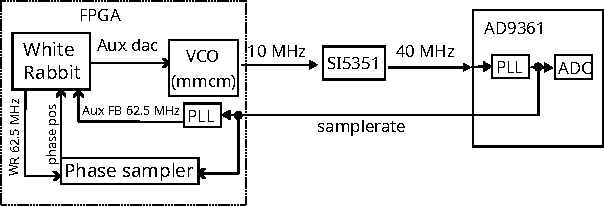
\includegraphics[width=\linewidth]{m2sdr_locksweep_fig.pdf}

\end{frame}

\begin{frame}[fragile]\frametitle{Auxiliary Locksweep}

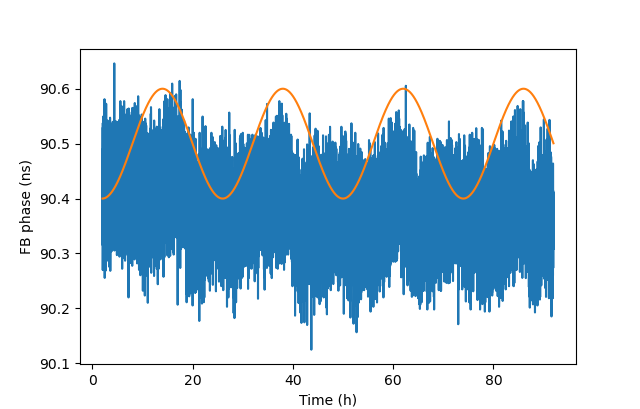
\includegraphics[width=\linewidth]{locksweep_phase_setpoint.png}
It  works!

\end{frame}



\begin{frame}[fragile]\frametitle{MMCM Phase Shifts Noise}
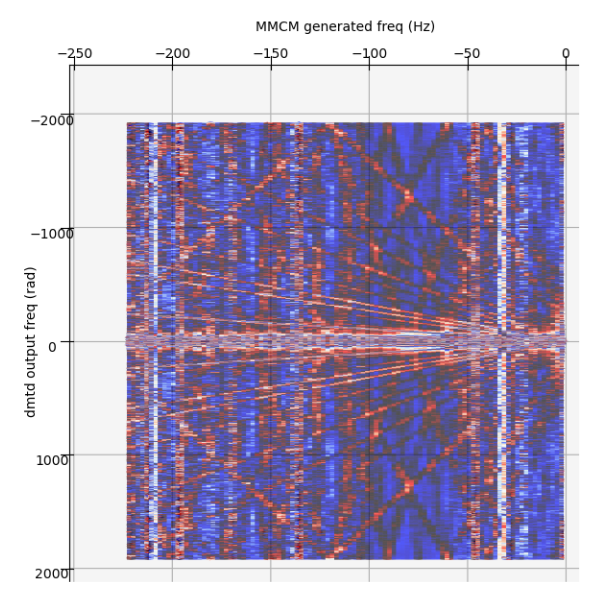
\includegraphics[width=\linewidth]{dmtd_spurs_by_mmcm_freq.png}
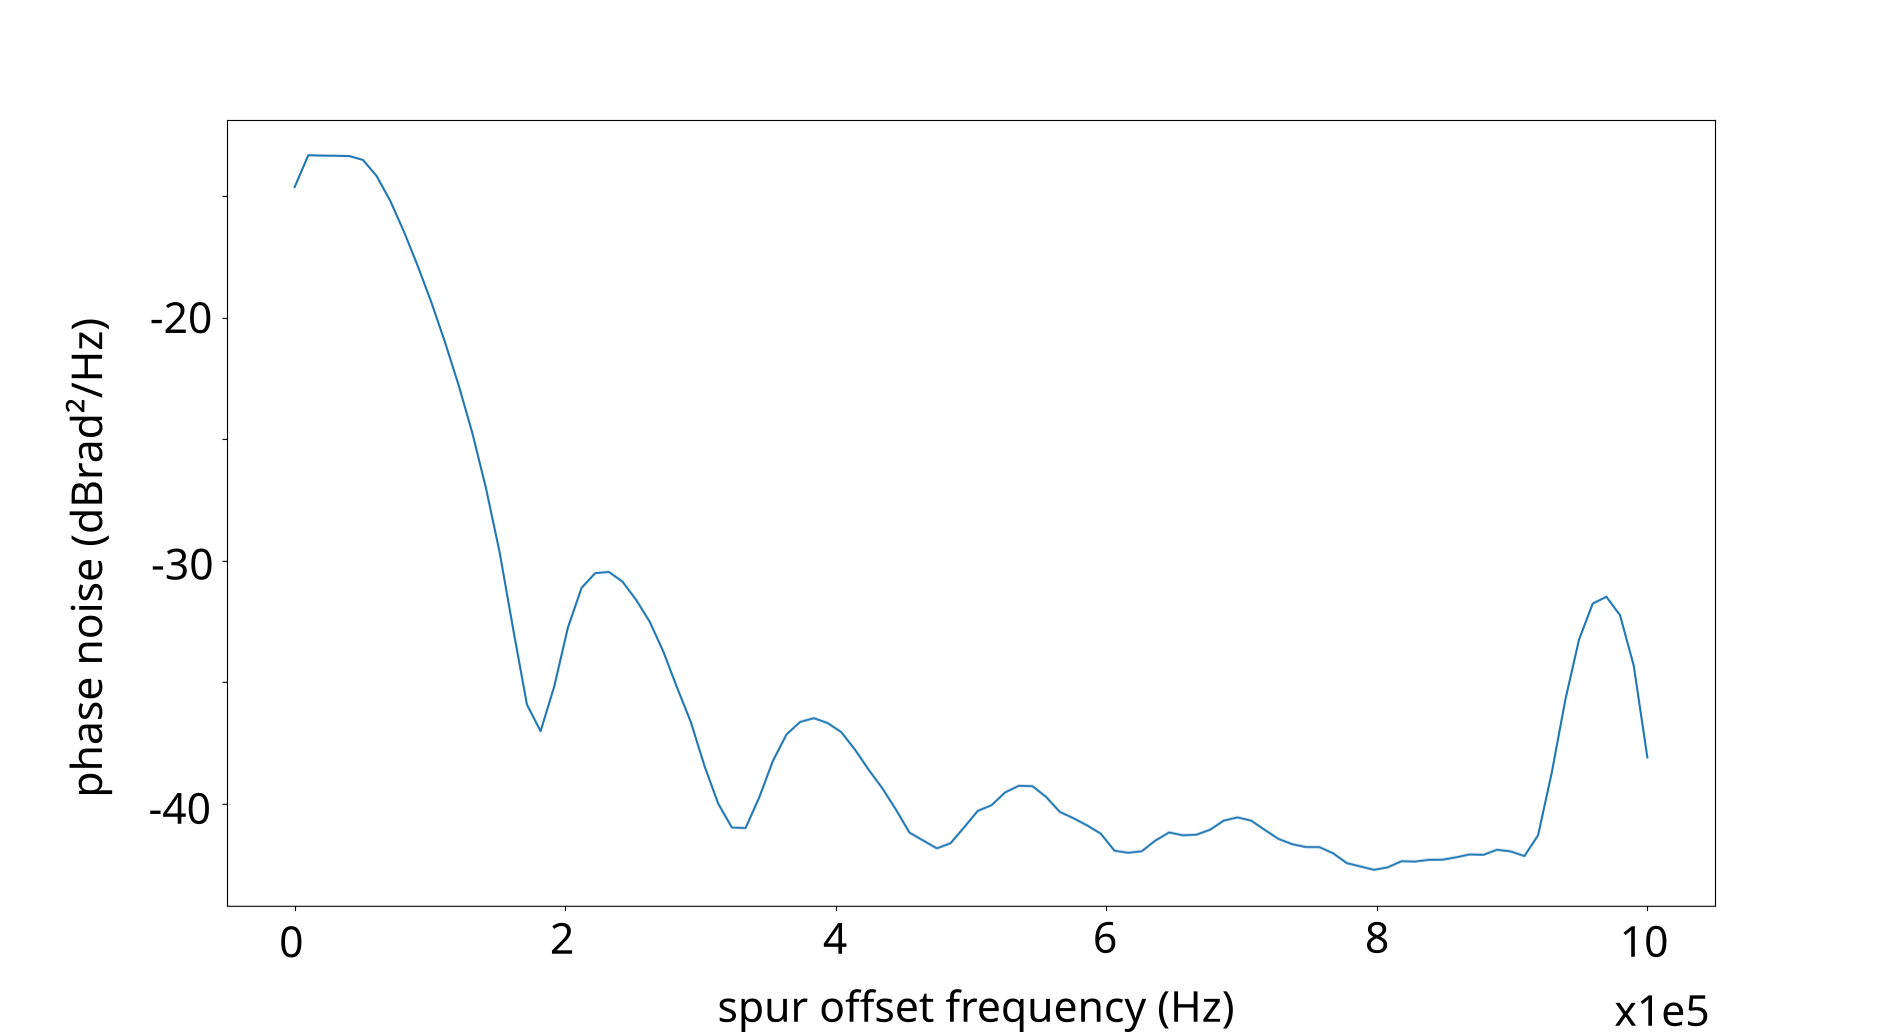
\includegraphics[width=\linewidth]{variance_by_spur_freq.png}

\end{frame}

\begin{frame}[fragile]\frametitle{Low Cost WR without MMCM tunning}

{Chained PLLs for helper}

{TXPI PPM for main tunning}

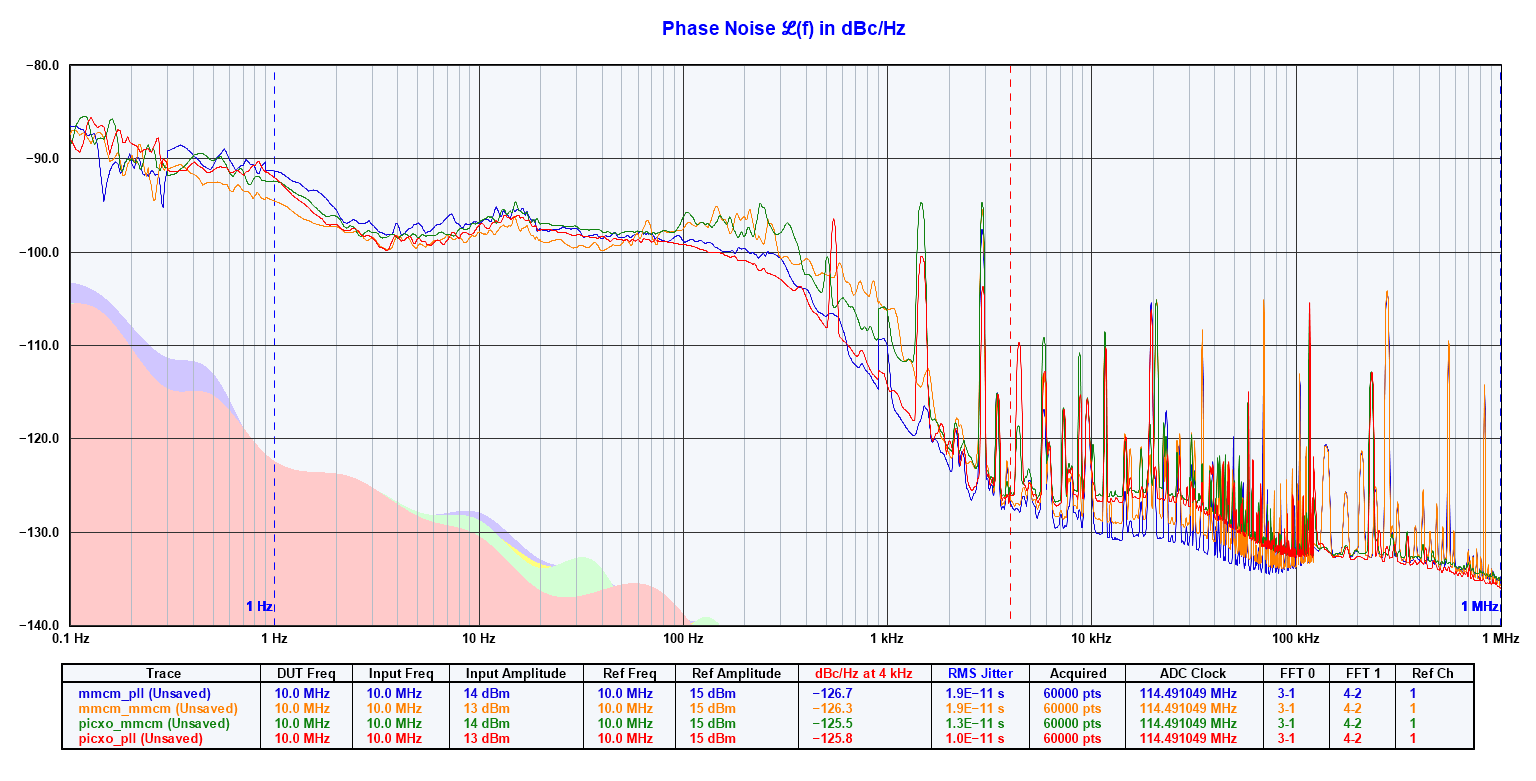
\includegraphics[width=\linewidth]{wr_alternative_clocking_comparison_correct_gain.png}

\end{frame}



\end{document}
